%!TEX root = avollmer.tex

\section{Results}

As stated before, the current pilot study serves as a proof of concept. We aimed at designing a setup allowing to study the processes involved in the formation of interaction protocols in asymmetric interaction with the particular constraint that the players could neither solve the task by themselves nor did they have access to any reward function.

Our first pilot study revealed a great potential in the use of our experimental method to study many aspects of communication relevant to HRI. With our setup, we will be able to study amongst others questions related to alignment, rhythm, contingency, and feedback, which have been in the focus of HRI research for some time \cite{kopp2010social,michalowski2007dancing,fischer2013impact,vollmer2014robots,pitsch2013robot,wrede2010appropriate}.

Surprisingly, while the construction task in this setup seems really challenging on paper and participants thought they would never succeed, a majority of the architect-builder pairs succeeded on building the correct construction. We analyzed a total of 17 experiments, of which 13 were successful and 4 failed. The average duration of the runs was 18 minutes ($M = 18~min, SD = 11~min$) with a minimum of 7 minutes and a maximum of 45 minutes.

In what follows, we showcase very first results supporting our claim that our setup can be used to study the co-construction of meaning in restricted, asymmetric interaction. We will first show one run of the game in detail which should give the reader an idea about what happens in an interaction with our setup and the richness and aptness of the data to consider a variety of research questions. Then, we will continue with presenting preliminary results on the negotiation of signal meanings and with describing observations of the builder behavior. We will conclude with mentioning interesting, additional considerations which are beyond the scope of this paper but will be subject of future work.

\subsection{One experiment in detail} 
\label{sec:case}
Figure~\ref{fig:timeline} brings together information about button presses (logs), their intended and interpreted meanings (found by the experimenters from their notes and observations of logs), and the builder's actions (builder video of the construction workspace) and makes clear the bidirectionality of the interaction. On the bottom of the figure, we see that the builder proposes blocks to the architect (blocks not belonging to the target structure in black, blocks belonging to it in gray) (cf. Subsection~\ref{sec:builder}) and on the top we see how the architect responds to the builder's actions in terms of button presses and meanings. Additionally, we see how the builder interprets these signals of button presses which he/she perceives as symbols on a screen (middle timeline of button presses and meanings) and how these interpretations and believes in turn again influence what the builder does next.

With respect to the meanings of the button presses, we observe the change of button meanings over the course of the interaction. The exact points in time when meaning changes occur have been matched to the button presses by hand and is therefore approximated. While this may be a problem for detailed analyses on a micro level, it is of little importance for the macro analysis presented here. During the first 4 minutes, the architect changes the intended meanings of signals many times and these meanings were not aligned with the builder's interpretation of signals. At 4 minutes, the architect presses all buttons at once, seemingly attempting to ask the builder to clear his/her mind and start over again. Right after this \emph{Reset} signal, the architect changes to one simple \emph{yes/no} strategy using button 1 and 6. On the builder's end, this Reset signal is followed by a pause of actions which hints at a direct confusion. It is only at 12 minutes into the game that the builder fully understands the intended meaning of the architect's button presses and can start joining two blocks correctly (green graph on the bottom). The experiment continues with the builder suggesting new blocks (bottom - black and gray events) and positions for new blocks (bottom - red and green events) one at a time which are validated or invalidated by the architect. After 19 minutes, the architect presses again all the buttons but this time with the aim of informing the builder that the construction is complete. The builder ended the experiment at that time. The \emph{End} signal was well interpreted by the builder as the interaction was going smoothly until that time and the few remaining blocks were rejected (bottom - black event at 19 min). The final construction was indeed the target one intended by the architect, hence resulting in a successful experiment.

%concluding sentence
Our setup allows studying the evolution of meanings associated to each button and put it in relation with the current context in the interaction.
We find that the constraints inherent to our setup allow analyzing communication, especially the interplay of individual actions and their interactional history, as well as their concrete timing, while lowering interactional complexity and thereby reducing communicative noise.

\begin{figure*}[!tb]
\centering
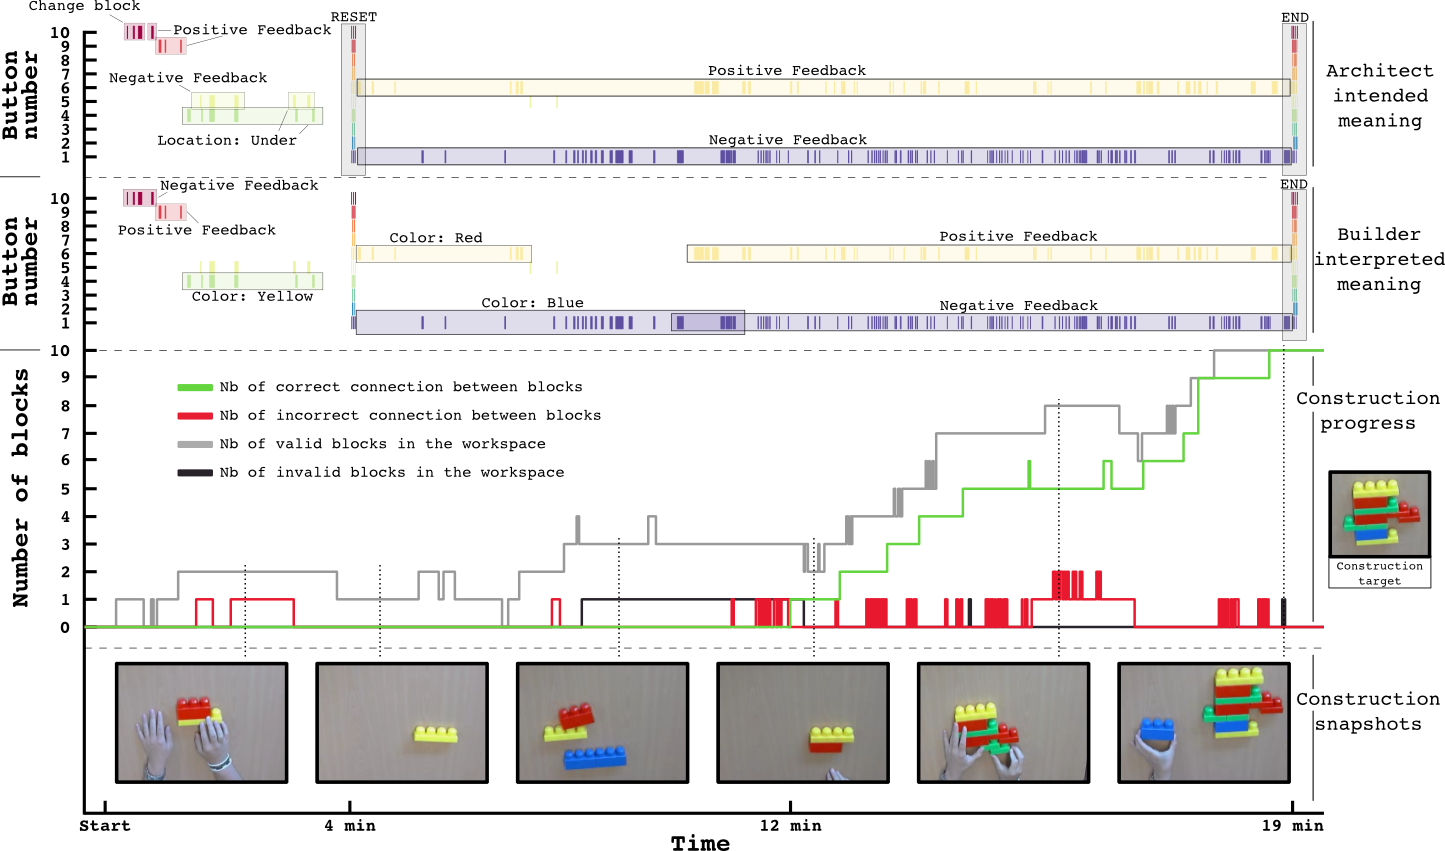
\includegraphics[width=\textwidth]{media/plots/timeline_with_visu}
\caption{Timeline for one experiment of an architect and a builder collaborating towards building the construction target (right hand side). 
The top and middle part show the timeline of button presses associated with the intended meaning from the architect (top) and the understood meaning from the builder (middle). There were 10 buttons, for which we logged all button presses for each experiment and here display all occurrences as colored dashes. Using the signal meanings participants reported during the game, the events are annotated with the meaning the architect intended or the builder understood. Events that are not annotated were not mentioned by the participants.
At the bottom, the figure additionally visualizes the progress made by the builder in assembling the target structure and also shows incorrect block propositions, joining of incorrect blocks and mistakes. These events were annotated by hand using the video annotation tool ELAN developed by the Max Planck Institute for Psycholinguistics, The Language Archive, Nijmegen, The Netherlands \cite{wittenburg2006elan}. A block proposition here started, when the transportation of the block towards the workspace ended and the block lay still on the table. It ended when the block was again picked up and subsequently removed from the workspace. These presentation events were classified into correct and incorrect propositions by determining whether the proposed block was part of the target structure. Equivalently, a joining event started, when two blocks were successfully joined at either a correct or incorrect position (again depending on whether the resulting configuration was part of the target structure). It ended before the first frame in which the two previously joined blocks were again pulled apart.}
\label{fig:timeline}
\end{figure*}

\subsection{Meanings} 

Architects and builders start the game without having agreed on specific meanings the buttons should convey. We start by studying the associated meanings obtained from our notes on signal meanings reported by builder and architect. They seemed to initially consider a large set of possible meanings, but, in the end, were able to agree primarily on only a limited number.

\textbf{Types of Meanings} 
When analyzing the notes on the participants' explanation of signal meanings (see Subsection \ref{sec:procedure}), we identified nine different categories of meanings:
\begin{enumerate}
    \item \textbf{Positive Feedback}
    \item \textbf{Negative Feedback}
    \item \textbf{End}: The construction is finished.
    \item \textbf{Reset}: Start over.
    \item \textbf{Guidance}: Instruction on what to do. It includes \emph{change, invert, revert, new block, continue, stack}. 
    \item \textbf{Color}: Reference to the color of a block. It includes \emph{yellow, blue, red, green}.
    \item \textbf{Size}: Reference to the size of a block. It includes \emph{small, medium, big}.
    \item \textbf{Location}: Reference to the location of a block. It includes \emph{under, above, left, right}.
    \item \textbf{Group}: Reference to a group of blocks. It includes \emph{in, out, group\_X}.
\end{enumerate}
Importantly, those categories where \textbf{not} suggested to the participants beforehand, but only identified by us in a posteriori analysis.

For each experiment, we determined if the architect or the builder considered each type of meaning (see Figure~\ref{fig:types_of_feedback}). In every single experiment, positive and negative feedback were considered on both architect and builder side. The \emph{End} meaning has been considered on both sides in 14 experiments. More concrete instructions such as \emph{Guidance, Color, Size, or Location} were less often considered, especially by the builder.

\begin{figure}[!ht]
  \begin{center}
      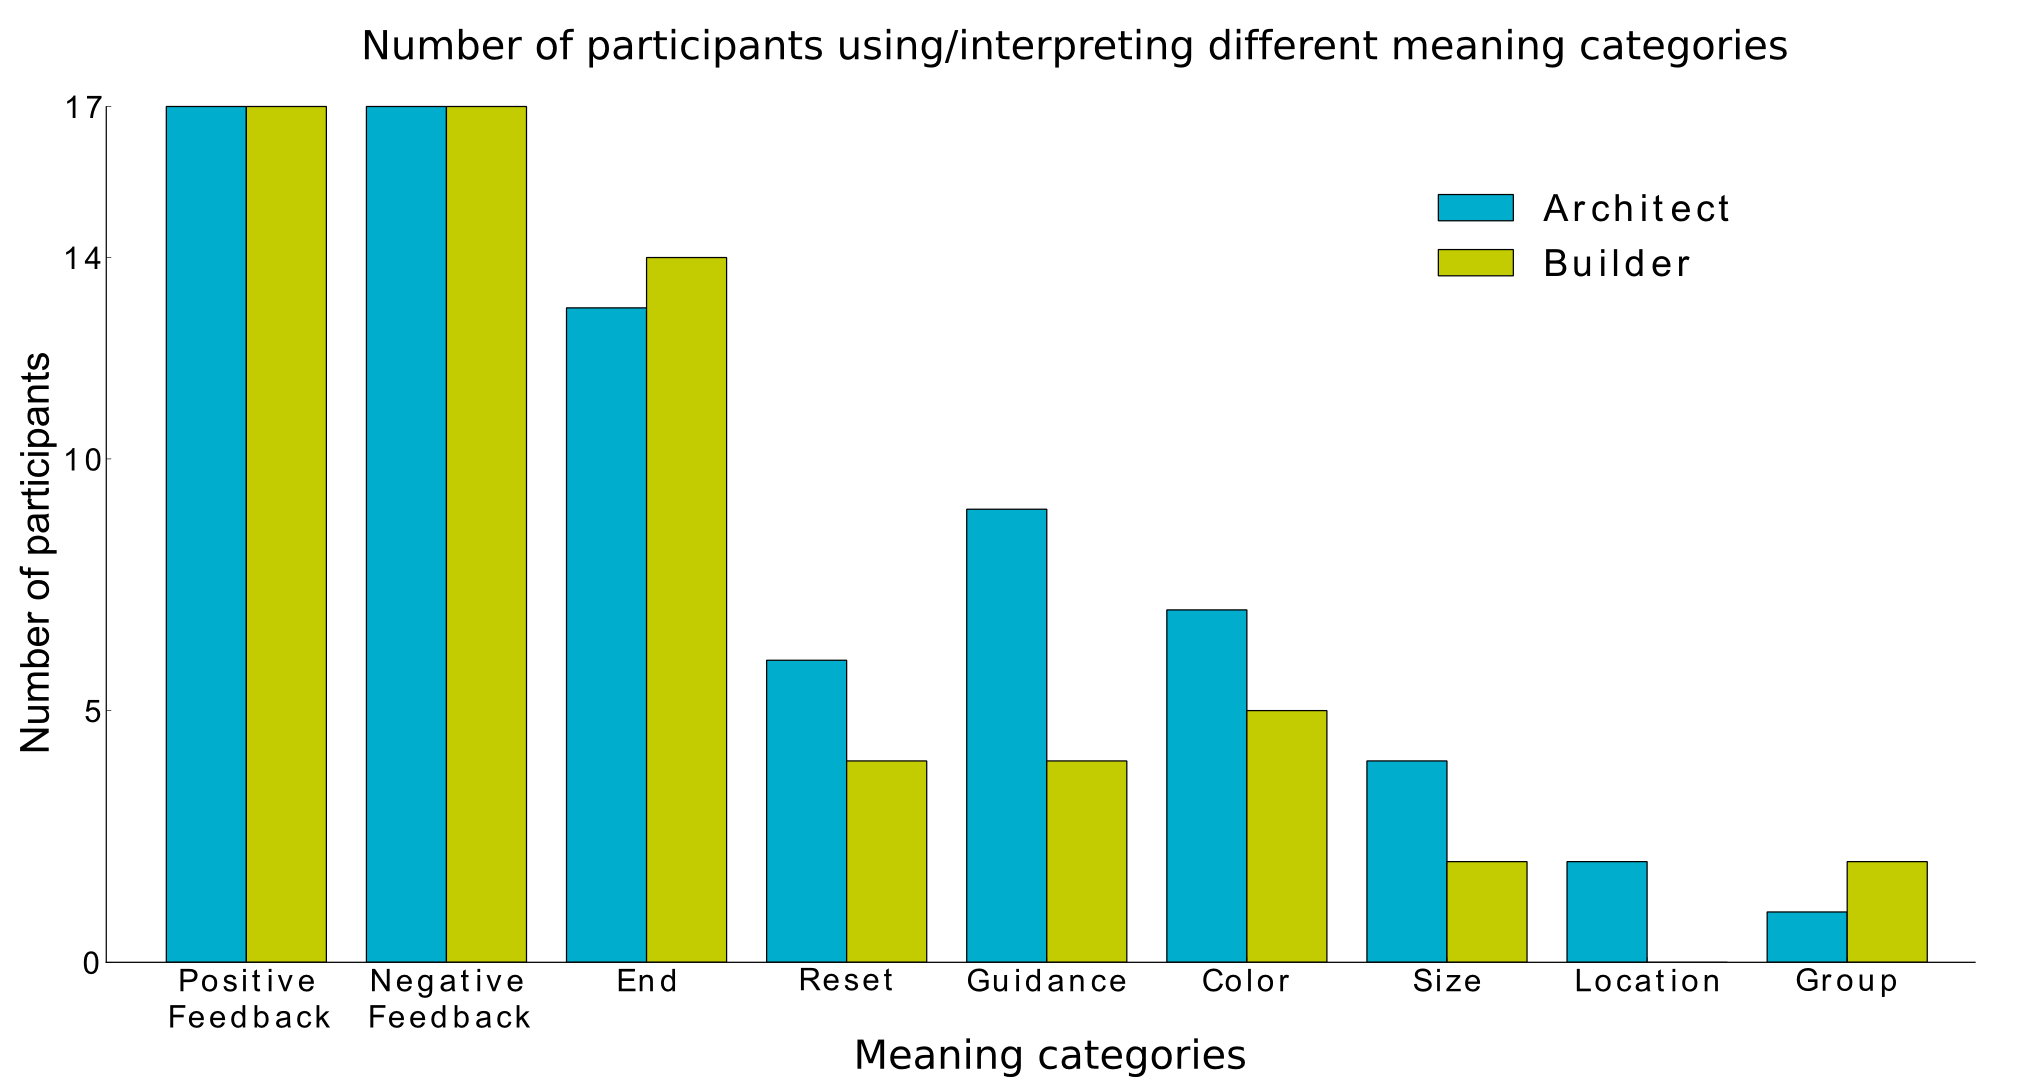
\includegraphics[width=\columnwidth]{media/plots/instruction_type}
      \caption{Number of participants that used (architect) or interpreted (builder) signals as conveying different types of meaning. All participants considered positive and negative feedback types of meaning.}
    \label{fig:types_of_feedback}
  \end{center}
\end{figure}

This is in line with the findings in \cite{griffiths2012bottom}, where \emph{``yes''} and \emph{``no''} were also identified to be among the most common types of signal meanings.

\textbf{Matching of meanings between architect and builder} Knowing which meaning categories were considered by each of the participants does not tell us if a particular pair of players understood each other. We therefore compared the associated meanings reported by architect and builder for all signals. Similarly to \cite{griffiths2012bottom}, we then determined the number of signals that were understood, misinterpreted, or ignored. We define signals which were understood as signals where both architect and builder agree on a common meaning. For signals which were misinterpreted, the builder reported a different associated meaning than the one the architect intended. The signals which were mentioned by the architect, but not by the builder, we counted as ignored signals. We then averaged the results for successful and failed experiments, see figure~\ref{fig:types_of_understanding}. For successful experiments, the average number of signals understood is $M = 3.6, SD = 0.7$ which mostly corresponds to \emph{Positive feedback, Negative feedback, End}, and occasionally \emph{Reset} when needed (see Figure~\ref{fig:understanding_per_feedback}). Interestingly for failed experiments, this number drops to $M = 1.3, SD = 1.1$, with a larger amount of signals misinterpreted and ignored.

\begin{figure}[!ht]
	\begin{center}
      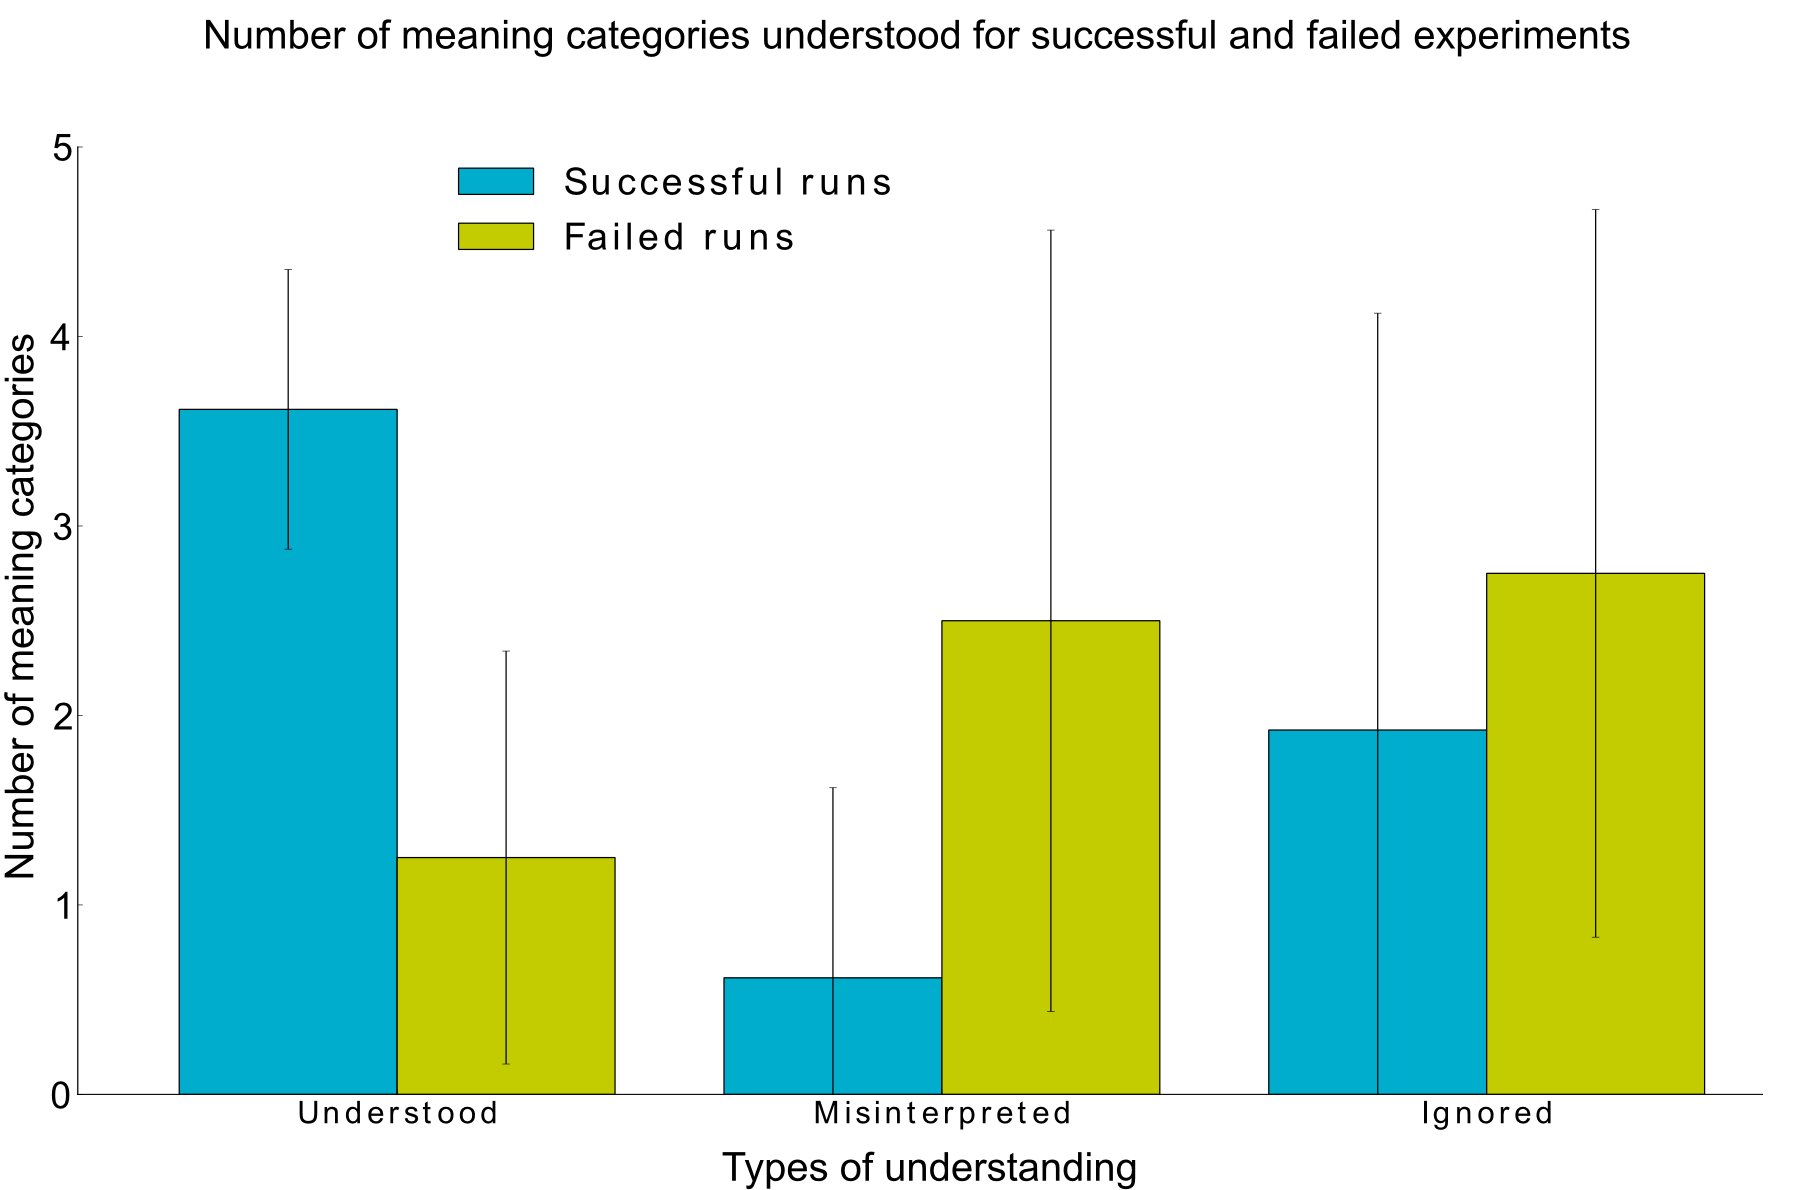
\includegraphics[width=\columnwidth]{media/plots/understood_std}
   		\caption{Distribution of meaning categories that were understood, misinterpreted, and ignored by the builders. Data average across all builders for successful (blue) and failed (yellow) experiments.}
      \label{fig:types_of_understanding}
   	\end{center}
\end{figure}

%\todo{Finally, figure~\ref{fig:understanding_per_feedback} is an attempt to describe what types of instruction where actually understood, misinterpreted, or ignored. It shows that \emph{Positive feedback}, \emph{Negative feedback}, \emph{End}, and \emph{Reset} are the most commonly understood instructions.

%\todo{JG: I have to check exactly how to explain that one, it is a bit weird to see wrt. Figure~\ref{fig:types_of_feedback} as the number for each instruction type is different, I have to check again why, if I remember well it is because I only consider it at the end of the experiment and only from the builder side but it is hard to remember}

\begin{figure}[!ht]
  \begin{center}
      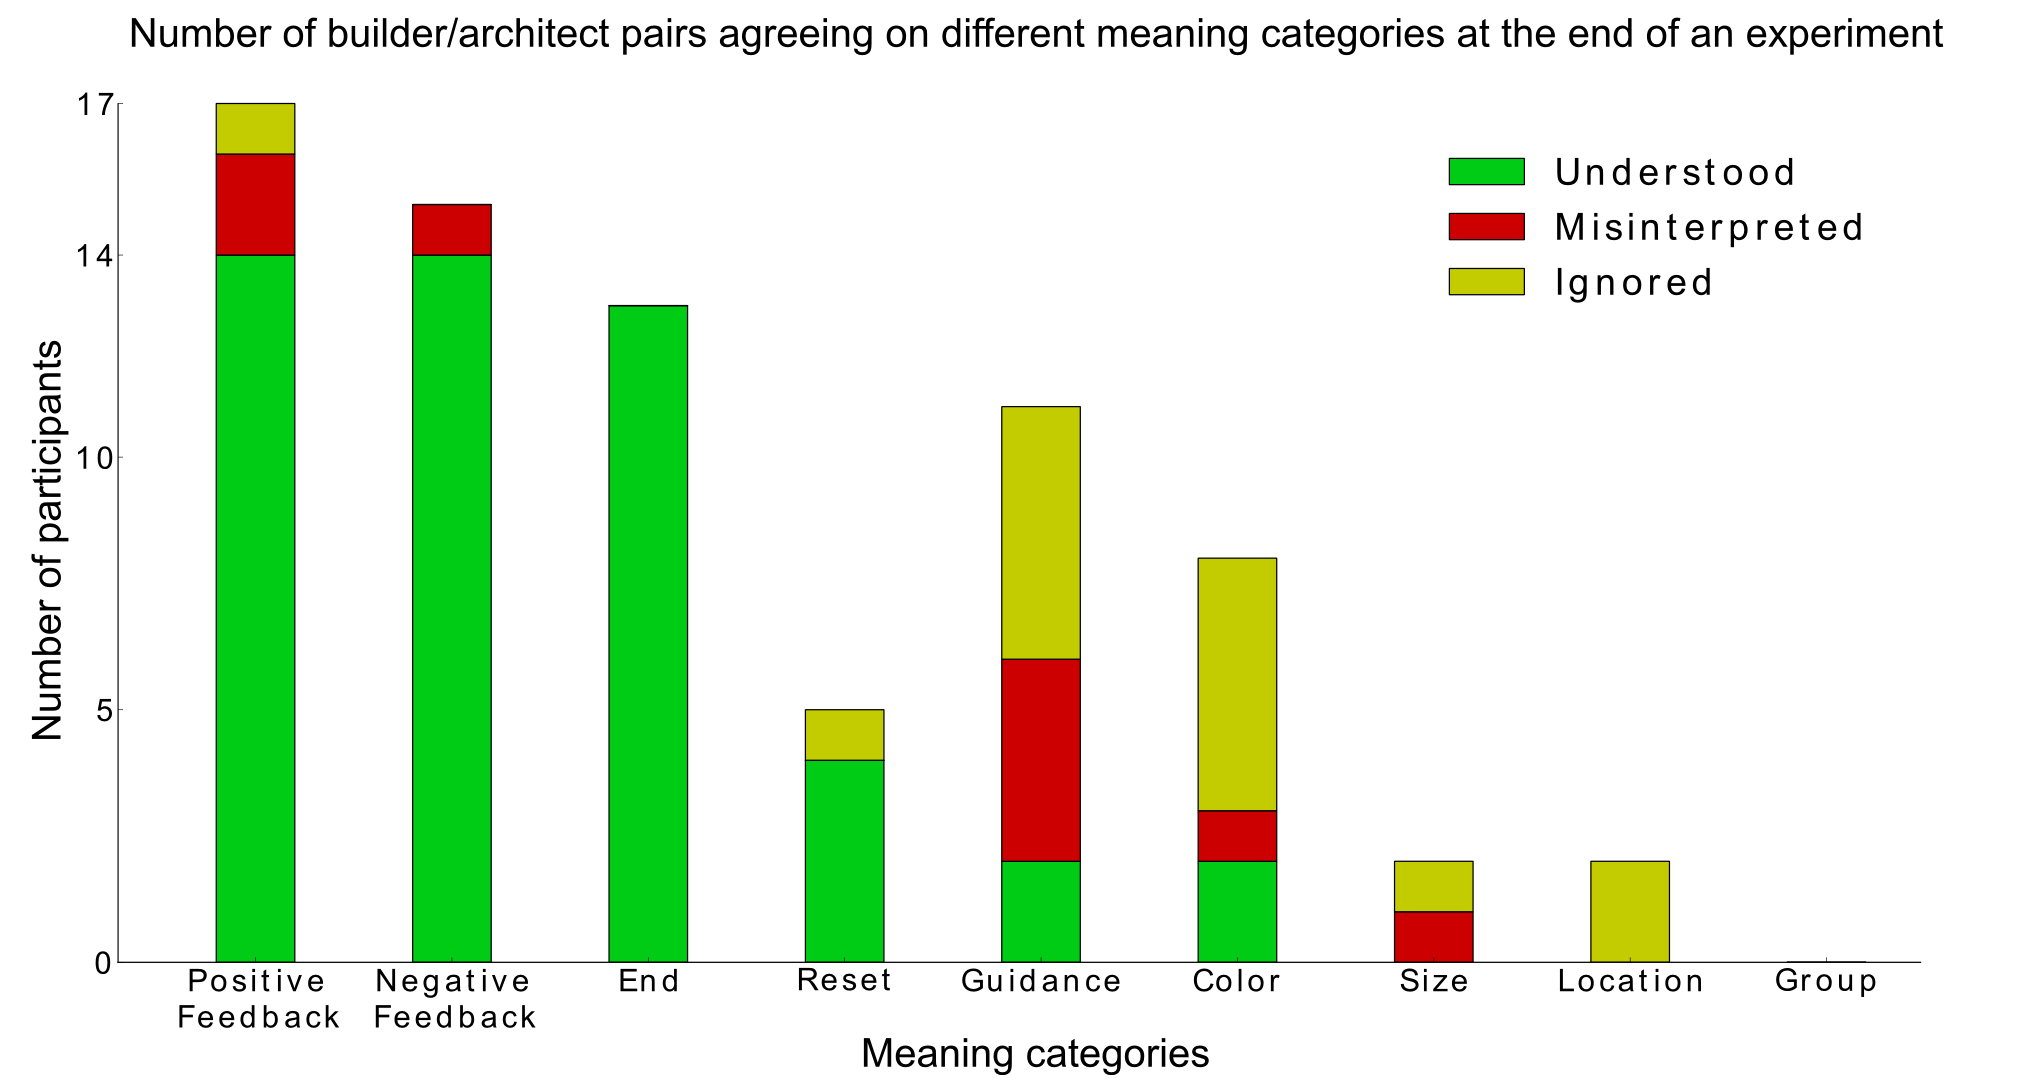
\includegraphics[width=\columnwidth]{media/plots/instruction_understood}
      \caption{Number of builder/architect pairs agreeing or disagreeing on different meaning categories at the end of an experiment.}
    \label{fig:understanding_per_feedback}
    \end{center}
\end{figure}

It seems that even though many different signal meanings are initially considered by the architect, the players agree only on very few specific ones (positive feedback, negative feedback and End). The question of what are the main factors determining which meanings are considered by participants arises.
This leads over to the next subsection in which we will consider the builder behavior to explore its role in which signal meanings are considered and in the ultimate outcome of the game.

\subsection{Builder Strategies}
\label{sec:builder}
For the builder, we aimed at identifying common actions across participants in an attempt to quantify the builders' strategies from the video data showing a top-down view of the workspace.
What follows is a description of observations on the builders' behaviors.

We identified two main strategies the builders embarked on (for an overview see Table~\ref{table:builder}). For these two strategies, the builders began by presenting only one block at a time. When they presented several blocks at once throughout the game, they did not seem to embark on a successful strategy. 

The most common strategy for builders was to determine one correct brick at a time and to subsequently join it with the already assembled structure (see Figure~\ref{fig:timeline}). Figure~\ref{fig:timeline} is a case example of one game/run of the study in which this strategy is used successfully.
The builders in $12$ (five first rounds and their five respective second rounds, one independent single first round, and one second round) of the $17$ runs pursued the same strategy. Only one game (a first round with a successful corresponding second round) of these $12$ failed. 

The other strategy was to find all blocks belonging to the target structure. Blocks identified as correct were not joined right away, but in a first step all blocks belonging to the target structure were determined and were then subsequently joined one at a time in a second step. This strategy also involved the presentation of only one block at a time and was eventually pursued by two builders who both started out with a different strategy involving the presentation of multiple blocks. 
One builder initially tried to find which forms belonged to the target structure. Ultimately, he then identified all blocks belonging to the target structure by one at a time dividing all blocks into two groups. This builder played in a second round, for which in its corresponding first round multiple blocks were presented at a time by the builder and the game failed.
Another builder at the beginning tried to elicit a label for either color or form from the architect. In this case, all blocks of one specific color or of one specific shape were presented at a time. This strategy was only pursued by one builder at the beginning of the game, but was not successful and then therefore discontinued in favor of the strategy of finding which blocks belong to the target structure. This builder played in a first round. In the corresponding second round, the builder embarked on the first strategy.

The remaining three builders (in three first rounds) also presented multiple blocks at once but the set of blocks presented did not have any common properties and seemed random. These builders did not have any apparent systematic strategy and their games did not come to a successful end.

 \begin{table}[h]
 \begin{tabular}{p{0.22\columnwidth}|p{0.22\columnwidth}|p{0.12\columnwidth}|p{0.12\columnwidth}|p{0.06\columnwidth}}
%
 \multicolumn{1}{m{0.22\columnwidth}|}{\centering Presentation of blocks} & \multicolumn{1}{m{0.22\columnwidth}|}{\centering Strategy} & \multicolumn{1}{m{0.12\columnwidth}|}{\centering Number of games} & \multicolumn{1}{m{0.12\columnwidth}|}{\centering Successful} & \multicolumn{1}{m{0.06\columnwidth}}{\centering Failed} \\ \hline
%
 \multicolumn{1}{m{0.22\columnwidth}|}{\centering Present one block at a time} & \multicolumn{1}{m{0.22\columnwidth}|}{\centering Find one block and join right away, repeat}                    & \multicolumn{1}{m{0.12\columnwidth}|}{\centering 12}              & \multicolumn{1}{m{0.12\columnwidth}|}{\centering 11}                         & \multicolumn{1}{m{0.06\columnwidth}}{\centering 1}                      \\ \cline{2-5}
% 
  & \multicolumn{1}{m{0.22\columnwidth}|}{\centering Find all blocks belonging to the structure, then start joining} & \multicolumn{1}{m{0.12\columnwidth}|}{\centering 2}                       & \multicolumn{1}{m{0.12\columnwidth}|}{\centering 2}                          & \multicolumn{1}{m{0.06\columnwidth}}{\centering 0} \\ \hline 
 %
 \multicolumn{1}{m{0.22\columnwidth}|}{\centering Present multiple blocks at a time} & \multicolumn{1}{m{0.22\columnwidth}|}{\centering No strategy}                               & \multicolumn{1}{m{0.12\columnwidth}|}{\centering 3}               & \multicolumn{1}{m{0.12\columnwidth}|}{\centering 0}                          & \multicolumn{1}{m{0.06\columnwidth}}{\centering 3}                     
 \end{tabular}
 \caption{}
 \label{table:builder}
 \end{table}
%
%\begin{table}[!ht]
%\centering
%
\includegraphics[width=0.9\columnwidth]{media/plots/table}
%\caption{}
%\label{table:builder}
%\end{table}
%
Taking a closer look at the four failed experiments, we find that in one of them, where the builder presented one block at a time, in the end the target construction was almost finished. Architect and builder understood each other, but what happened is that an early mistake in the position of one block was not signaled and thus corrected by the architect right away. He waited until the rest of the structure was completed and then tried to address the mistake by means of the introduction of a new signal. This new signal was interpreted by the builder as an End signal, leading to the end of the game with one block in a position next to the target one.
With respect to the other failed experiments, the structure at the time the game ended was far from the target construction and there was no noticeable progress in all three cases.

Whereas, with the current data and analysis, we cannot yet draw any conclusions, still this observation suggests that the way the builders propose next steps and ask for information from the architect is important for the success of the game. Builders seem to build frames and create slots for the architect's input. These frames form the context which shapes the interpretation of the signals. This is similar to how in other cases of asymmetric or restricted communication, as for example in interactions with preverbal infants or in interactions with impaired persons, people provide frames to understand what their interaction partners with their different or limited conversational abilities want to communicate \cite{ochs1979propositions, goodwin1995co}.

\subsection{Additional Observations}
This subsection briefly indicates interesting, additional observations we made with our pilot study, as well as interesting considerations for future work.

First of all, we would like to state that the history of the interaction is crucial for understanding meanings. A person who has not witnessed the course of the interaction, is not able to fill in and complete the task without special instructions. We observe a phase of confusion and negotiation at the beginning of the interactions and after that a completion phase in which signal meanings have been constituted. The latter seems to be characterized by smooth, consistent patterns. In the initial phase of negotiation, we observed instances where the players adapted to their partners by changing the meaning of a button when they noticed the other player understands it differently (cf. Figure~\ref{fig:timeline} in Subsection~\ref{sec:case}). There were for example cases in which the meaning of signals meaning yes and no were reversed.
In contrast, we also observed that some players, both architects and builders, insisted on their strategies, even though the interaction with their respective partner did not work, i.e. they did not agree on any meaning and the task did not progress. Thus, there seem to be leaders and followers in terms of strategies, which could be personality-dependent, but could also manifest their ability to employ a theory of mind.

% We also noticed that builder strategies were adopted in a second round of the game, when builder and architect switched roles.
We also note that when builder and architect switched roles after a first round, their behaviors and performances were influenced (e.g., builder strategies were adopted across rounds). If a second round was systematically part of the experimental procedure, it would be interesting to see whether participants succeed faster in the second game they play with reversed roles and if they adopt similar strategies.

Another interesting aspect concerns timing, not only at which points in time the architect gives feedback and instructions, but also the interplay between the builder's and the architect's actions. The rhythm of the interaction partners' actions might be an important low-level feature in determining whether a certain signal means positive or negative feedback.

%opportunistic co-construction?
While the above points are highly relevant and worth investigating, their examination is beyond the scope of this paper and will be subject of future work.
